\documentclass{standalone}
\usepackage{tikz}
\usetikzlibrary{matrix,arrows,decorations.pathmorphing,decorations.pathreplacing,calc,positioning}
\usepackage{xcolor}
% all other packages and stuff you need for the picture
\newcommand{\myunit}{0.65 cm}
\newcommand{\myraise}{3pt}
\tikzset{
    lpltsty/.style={decorate, decoration = {brace,mirror,raise=3pt,amplitude=5pt}},
    namesty/.style={pos=0.5,below=7pt},
    scalarsty/.style={draw,fill=white,rectangle,minimum size=\myunit,anchor=center},
    indexsty/.style={fill,fill=white,rectangle,minimum width=\myunit,anchor=center},
    touchsty/.style={fill,fill=red,rectangle,minimum size=\myunit},
    ycsty/.style={fill,fill=yellow,rectangle,minimum size=\myunit},
    brcsty/.style={fill,fill=brown,rectangle,minimum size=\myunit},
    blcsty/.style={fill,fill=cyan!20,rectangle,minimum size=\myunit},
    becsty/.style={fill,fill=beige,rectangle,minimum size=\myunit},
    ocsty/.style={fill,fill=orange,rectangle,minimum size=\myunit},
    whclsty/.style={fill,fill=white,rectangle,minimum size=\myunit},
    zcsty/.style={fill,fill=white,rectangle,minimum size=\myunit,text=zerogray},
    nzsty/.style={fill,fill=black,rectangle,minimum size=\myunit,text=white},
    rcsty/.style={fill,fill=purple,rectangle,minimum size=\myunit},
    pcsty/.style={fill,fill=pink,rectangle,minimum size=\myunit},
    lcsty/.style={fill,fill=blue,rectangle,minimum size=\myunit},
    bcsty/.style={fill,fill=black,rectangle,minimum size=\myunit, text=white},
    hlsty/.style={draw=red},
}


\colorlet{zerogray}{gray!25}
\colorlet{beige}{brown!70}

\newcommand{\ylcl}{|[ycsty]|1}
\newcommand{\recl}{|[rcsty]|2}
\newcommand{\picl}{|[pcsty]|3}
\newcommand{\blcl}{|[blcsty]|1}
\newcommand{\brcl}{|[brcsty]|2}
\newcommand{\becl}{|[becsty]|3}
\newcommand{\orcl}{|[ocsty]|4}
\newcommand{\bkcl}{|[bcsty]|5}
\newcommand{\whcl}{|[whclsty]|0}
\newcommand{\zecl}{|[zcsty]|0}

\newcommand{\formatscale}{0.5}
\newcommand{\matrixscale}{0.69}
\begin{document}

\resizebox{\linewidth}{!}{%
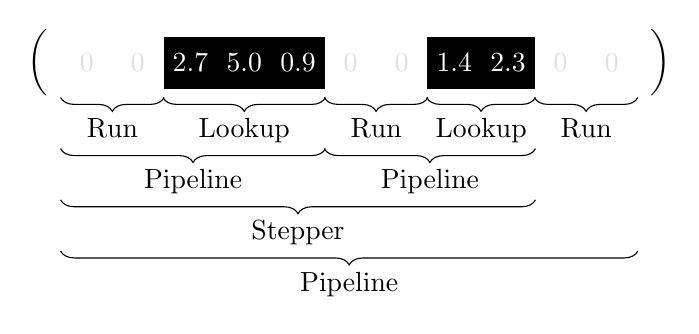
\begin{tikzpicture}[>=latex]
  \matrix (A) [matrix of math nodes,
              nodes = {whclsty},
              left delimiter  = (,
              right delimiter = ),
              ampersand replacement=\&] at (0,0)
  {
  \zecl \& \zecl \& |[nzsty]|2.7 \& |[nzsty]|5.0 \& |[nzsty]|0.9 \& \zecl \& \zecl \& |[nzsty]|1.4 \& |[nzsty]|2.3 \& \zecl \& \zecl \\
  };

  \draw[lpltsty] ([yshift=-0*\myunit]A-1-1.south west) -- ([yshift=-0*\myunit]A-1-2.south east) node[namesty]{Run};
  \draw[lpltsty] ([yshift=-0*\myunit]A-1-3.south west) -- ([yshift=-0*\myunit]A-1-5.south east) node[namesty]{Lookup};
  \draw[lpltsty] ([yshift=-0*\myunit]A-1-6.south west) -- ([yshift=-0*\myunit]A-1-7.south east) node[namesty]{Run};
  \draw[lpltsty] ([yshift=-0*\myunit]A-1-8.south west) -- ([yshift=-0*\myunit]A-1-9.south east) node[namesty]{Lookup};
  \draw[lpltsty] ([yshift=-0*\myunit]A-1-10.south west) -- ([yshift=-0*\myunit]A-1-11.south east) node[namesty]{Run};
  \draw[lpltsty] ([yshift=-1*\myunit]A-1-1.south west) -- ([yshift=-1*\myunit]A-1-5.south east) node[namesty]{Pipeline};
  \draw[lpltsty] ([yshift=-1*\myunit]A-1-6.south west) -- ([yshift=-1*\myunit]A-1-9.south east) node[namesty]{Pipeline};
  \draw[lpltsty] ([yshift=-2*\myunit]A-1-1.south west) -- ([yshift=-2*\myunit]A-1-9.south east) node[namesty]{Stepper};
  \draw[lpltsty] ([yshift=-3*\myunit]A-1-1.south west) -- ([yshift=-3*\myunit]A-1-11.south east) node[namesty]{Pipeline};
\end{tikzpicture}%
} 
\end{document}